
\documentclass[dvipdfmx]{beamer}
\AtBeginShipoutFirst{\special{pdf:tounicode EUC-UCS2}}

\usetheme{Madrid}
\usecolortheme{default}
\setbeamerfont{frametitle}{size=\large,series=\bfseries}
\setbeamertemplate{navigation symbols}{}
\setbeamertemplate{footline}[frame number]
\setbeamertemplate{section in toc}[circle]
\setbeamertemplate{blocks}[rounded][shadow=true]

\definecolor{character}{RGB}{0,0,0} %文字
\definecolor{background}{RGB}{245,245,245} %背景
\setbeamercolor{Normal text}{bg=background, fg=character}

\definecolor{mathFormula}{RGB}{53,121,53} %数式
\setbeamercolor{math text}{fg=mathFormula}

\definecolor{alertColor}{RGB}{255,70,70} %alert
\setbeamercolor{alerted text}{fg=alertColor}

\definecolor{blockAlertColor}{RGB}{0,0,0} %alertblock内の文字
\setbeamercolor{block body alerted}{fg=blockAlertColor}

\definecolor{headColor}{RGB}{52,38,89} %見出しカラー
\setbeamercolor{structure}{fg=headColor}
\setbeamercolor{subsection in toc}{fg=headColor}

\usepackage[absolute,overlay]{textpos}
\setbeamercovered{dynamic}
% \usepackage[colorgrid,gridunit=pt,texcoord]{eso-pic}


% \mathversion{bold}
% \usefonttheme[onlymath]{serif}
% 文字フォント設定
% \setbeamertemplate{blocks}[rounded] % Blockの影を消す
% \mathversion{bold} %数式を太字に
\usefonttheme{professionalfonts}% 数式用フォント
\setbeamertemplate{items}[ball] % itemize 変更
\renewcommand{\kanjifamilydefault}{\gtdefault}  % 日本語をゴシック体に
\renewcommand{\familydefault}{\sfdefault} %英字をサンセリフに
\newcommand{\argmin}{\mathop{\rm arg~min}\limits}
%\renewcommand{\familydefault}{\rmdefault} %英字をローマンに
%\setbeamertemplate{section in toc}[square] %目次を球体から四角へ
% \newtheorem{remark}[theorem]{Remark}
% \newtheorem{observation}[theorem]{Observation}


\title{並列機械モデルにおける\\最大待ち時間最小化問題の計算論的分析}
\author{天本 祐希}
\institute{宋研究室}
\date{\today}

%%%%%%%%%%%%%%%%%%%%%%%%%%%%%%%%%%%%%%%%%%%%%%%%%%%%%%%%%%%%%%%%%%%
\AtBeginSection[]{
\begin{frame}{目次}
  % \tableofcontents
  \tableofcontents[currentsection,currentsubsection,
  hideothersubsections,
  sectionstyle=show/shaded,
  ]
  \end{frame} %目次スライド
  }
  %%%%%%%%%%%%%%%%%%%%%%%%%%%%%%%%%%%%%%%%%%%%%%%%%%%%%%%%%%%%%%%%%%%
  \begin{document}
  \maketitle
  %%%%%%%%%%%%%%%%%%%%%%%%%%%%%%%%%%%%%%%%%%%%%%%%%%%%%%%%%%%%%%%%%%%
  \begin{frame}{目次}
    \tableofcontents
    \end{frame} %目次スライド
    \section{計算論的分析とは}
    \begin{frame}{計算論的分析とは}
      \begin{block}{}

      \end{block}
    \end{frame}

    \section{研究背景}
    \begin{frame}{研究背景:Web サービスにおける処理の流れと問題}
      \begin{figure}[h]
        \centering
        \includegraphics<1>[width=12cm]{figure/server1.pdf}
        \includegraphics<2>[width=12cm]{figure/server2.pdf}
        \includegraphics<3>[width=12cm]{figure/server3.pdf}
        \includegraphics<4>[width=12cm]{figure/server4.pdf}
      \end{figure}

      \begin{block}{問題}
        \uncover<4->{
        Web サービスを運用している会社では,運用しているサービスの応答が遅いと,顧客離れやクレームの被害を受けることがある.そのため,計算サーバーの応答の早さは重要である.
        }
      \end{block}

    \end{frame}

    \begin{frame}{研究背景:スケジューリング問題との対応}
      \begin{block}{研究背景:スケジューリング問題との対応}
        Web サービスの問題を解決する方法の 1 つとして,\alert{タスクが到着してから,処理されるまでの時間を短くする}方法が挙げられる.計算サーバーにおける各時間は以下に対応する.つまり,計算サーバーへのタスク割り当ては,スケジューリング問題として捉えることができる.
        \begin{itemize}
          \item タスクの到着時刻とは,\alert{処理開始可能時刻}に対応する.
          \item タスクが到着してから,タスクの処理が開始されるまでの時間とは,\alert{待ち時間}に対応する.
        \end{itemize}
        \alert{最大待ち時間最小化問題(SWT)}は,処理開始可能時刻を制約とし,最大の待ち時間の最小化を目的とするスケジューリング問題として捉えることができる.
      \end{block}

      \begin{block}{研究目的}
        機械モデルおよび機械数に着目し,問題の難しさに影響を与える特徴を明らかにする.
        また,SWT の計算複雑さに基づいて,解法の提案を行う.
      \end{block}

    \end{frame}
    %%%%%%%%%%%%%%%%%%%%%%%%%%%%%%%%%%%%%%%%%%%%%%%%%%%%%%%%%%%%%%%%%%%
    % \section{定式化}
    % \subsection{最大待ち時間最小化問題の定式化}
    % \begin{frame}{定式化:最大待ち時間最小化問題}
    %   \begin{itemize}
    %     \item {無関連並列機械モデルにおいて,SWT を\alert{決定問題}として定義する.}
    %     \item {決定問題は,インスタンスと問題によって定義され,決定問題は判定とし
    %     て Yes または No のいずれかを持つ.}
    %   \end{itemize}
    %   \begin{block}{入力}
    %     \begin{itemize}
    %       \item {ジョブの集合 $\mathcal{J} = \{J_1,J_2,\ldots,J_n\}$}
    %       \item {無関連機械の集合 $\mathcal{M} = \{M_1,M_2,\ldots,M_m\}$}
    %       \item {ジョブの処理開始可能時刻を返す関数 $r : \mathcal{J} \to \mathbb{N}$}
    %       \item {ジョブの処理時間を返す関数 $p : \mathcal{J} \times \mathcal{M} \to \mathbb{N}$}
    %       \item {待ち時間 $w$}
    %     \end{itemize}
    %   \end{block}
    % \end{frame}
    %
    % \begin{frame}{定式化:最大待ち時間最小化問題}
    %   \begin{block}{問題}
    %     以下の条件を満たす $A : \mathcal{J} \to \mathcal{M}$ と $s : \mathcal{J} \to \mathbb{N}$ の対 $(A,s)$ が存在するか?
    %     \begin{itemize}
    %       \item {$\forall J \in \mathcal{J}\big[s(J) \ge r(J) \big]$}
    %       \begin{itemize}
    %         \item {各ジョブは処理開始可能時刻以降に処理を開始する.}
    %       \end{itemize}
    %       \item {$\forall J, J' \in \mathcal{J}\ \Big[ \big[J\ne J' \land A(J) = A(J')\big] \Rightarrow [s(J), s(J)+p(J,A(J))) \cap[s(J'), s(J')+p(J', A(J'))) = \emptyset \Big]$}
    %       \begin{itemize}
    %         \item {各機械は同時に複数のジョブを処理しない.}
    %         \item {各ジョブの処理を開始すると,完了するまで中断しない.}
    %       \end{itemize}
    %       \item {$\max\big\{s(J) - r(J) \mid J \in \mathcal{J}\big\} \le w$}
    %       \begin{itemize}
    %         \item {ジョブの処理開始可能時刻からその処理を開始するまでの待ち時間は $w$ 以下.}
    %       \end{itemize}
    %     \end{itemize}
    %   \end{block}
    % \end{frame}

    \begin{frame}{定式化:最大待ち時間最小化問題}
      \begin{block}{機械モデル}
        ジョブを処理する機械の台数について
        \begin{itemize}
          \item 1 つの機械で処理を行う\alert{単一機械モデル},
          \item 複数の機械で処理を行う\alert{並列機械モデル},
        \end{itemize}
        に分類される.
        本研究では,並列機械モデルの中で,すべての機械の性能が等しい\alert{同一並列機械モデル}とジョブと機械の組み合わせによって処理時間が異なる\alert{無関連並列機械モデル}を扱う.
      \end{block}

      以下,無関連並列機械モデルにおける SWT を定式化する.
      SWT のインスタンスを 4 項組 $(\mathcal{J}, \mathcal{M}, r, p)$ で表す.
      \begin{block}{入力}
        \begin{itemize}
          \item {ジョブの集合 $\mathcal{J} = \{J_1,J_2,\ldots,J_n\}$}
          \item {無関連機械の集合 $\mathcal{M} = \{M_1,M_2,\ldots,M_m\}$}
          \item {ジョブの処理開始可能時刻を返す関数 $r : \mathcal{J} \to \mathbb{N}$}
          \item {ジョブの処理時間を返す関数 $p : \mathcal{J} \times \mathcal{M} \to \mathbb{N}$}
        \end{itemize}
      \end{block}
    \end{frame}

    \setbeamercolor{math text}{fg=white}
    \begin{frame}{定式化:最大待ち時間最小化問題}
      \begin{block}{解:スケジュール $(A,s)$}
        \setbeamercolor{math text}{fg=mathFormula}
        以下の条件を満たす $A : \mathcal{J} \to \mathcal{M}$ と $s : \mathcal{J} \to \mathbb{N}$ の 2 項組 $(A,s)$.
        \begin{itemize}
          \item {$\forall J \in \mathcal{J}\big[s(J) \ge r(J) \big]$}
          \begin{itemize}
            \item {各ジョブは処理開始可能時刻以降に処理を開始する.}
          \end{itemize}
          \item {$\forall J, J' \in \mathcal{J}\ \Big[ \big[J\ne J' \land A(J) = A(J')\big] \Rightarrow [s(J), s(J)+p(J,A(J))) \cap[s(J'), s(J')+p(J', A(J'))) = \emptyset \Big]$}
          \begin{itemize}
            \item {各機械は同時に複数のジョブを処理しない.}
            \item {各ジョブの処理を開始すると,完了するまで中断しない.}
          \end{itemize}
        \end{itemize}
      \end{block}

      \setbeamercolor{math text}{fg=white}
      \begin{block}{目的関数:最大待ち時間 $W_{\max}$}
        \setbeamercolor{math text}{fg=mathFormula}
        \begin{itemize}
          \item $\varphi(A,s) = {\displaystyle \max_{J \in \mathcal{J}}\{s(J) - r(J)\}}$
          \begin{itemize}
            \item すべてのジョブの中で,ジョブの処理開始可能時刻と処理開始時刻の差が最大のもの.
          \end{itemize}
        \end{itemize}
      \end{block}
      \setbeamercolor{math text}{fg=mathFormula}
      \setbeamertemplate{items}[default]
      \begin{itemize}
        \item 最大待ち時間 $W_{\max}$ の最小化を目的とするスケジューリング問題
      \end{itemize}
    \end{frame}

    \setbeamertemplate{items}[ball]
    \setbeamercolor{math text}{fg=mathFormula}
    \begin{frame}{定式化:最大待ち時間最小化問題(決定問題)}
      SWT を\alert{決定問題}として定義する.
      決定問題は,インスタンスと問題によって定義され,判定として \alert{Yes} または \alert{No} のいずれかを持つ.
      \begin{block}{入力}
        \begin{itemize}
          \item SWT のインスタンス $(\mathcal{J}, \mathcal{M}, r, p)$
          \item {待ち時間 $w$}
        \end{itemize}
      \end{block}

      \begin{block}{問題}
        \begin{itemize}
          \item {$\max\big\{s(J) - r(J) \mid J \in \mathcal{J}\big\} \le w$}
          \begin{itemize}
            \item {ジョブの処理開始可能時刻からその処理を開始するまでの待ち時間は $w$ 以下.}
          \end{itemize}
        \end{itemize}
      \end{block}
    \end{frame}

    \subsection{\textsc{3-SATISFIABILITY} の導入}
    \begin{frame}{定式化:${\textcolor{white}{\mbox {\sc 3-SATISFIABILITY}}}$}
      \textsc{3-SATISFIABILITY (3-SAT) } は決定問題の 1 つで,この問題は NP 完全であることが知られている.
      \begin{block}{\textsc{3-SATISFIABILITY}}
        \begin{description}
          \item[インスタンス:] $(X,H)$
          \vspace{-2mm}
        \end{description}
        \begin{itemize}
          \item ブール型の変数集合 $X=\{x_1,x_2,\dots ,x_n\}$
          \begin{itemize}
            \item リテラルの集合 $L_X = X \cup \{\bar x \mid x \in X\}$
            \begin{itemize}
              \item $X$ と $X$ の各要素の論理否定をとった変数の集合
            \end{itemize}
          \end{itemize}
          \item 3 つのリテラルからなる節 $h$ の集合 $H$
          \begin{itemize}
            \item $H \subseteq 2^{L_X}$ s.t. $\forall h \in H \big[|h| = 3\big]$
          \end{itemize}
        \end{itemize}
        \begin{description}
          \setlength{\leftskip}{-8mm}
          \item[問題:] 以下を満たす真理値割り当て $f : X \to \{0,1\}$ が存在するか?
        \end{description}
        $$\displaystyle \bigwedge_{h \in H} \bigg(\bigvee_{x \in h}f(x) \lor \bigvee_{\bar x \in h}\lnot f(x) \bigg) = 1$$
      \end{block}

      例えば,$X = \{x_1,x_2,x_3\}$,$H = \big\{ \{x_1, x_2, \bar x_3\}, \{\bar x_1, \bar x_2,\bar x_3\}\big\}$ のとき,
      $f(x_1) = 1, f(x_2) = 0, f(x_3) = 0$ が存在するので,判定は Yes となる.
    \end{frame}
    %%%%%%%%%%%%%%%%%%%%%%%%%%%%%%%%%%%%%%%%%%%%%%%%%%%%%%%%%%%%%%%%%%%
    \section{多項式還元とは}
    \begin{frame}{多項式還元とは:還元の流れ}
      \begin{tabular}{cc}
        \begin{minipage}[c]{0.5\hsize}
          \begin{block}{NP 完全}
            ある問題が NP 完全であることを示すには,以下が成立することを示す.
            \begin{itemize}
              \item 問題がNPに属す.
              \item 問題がNP困難である.
            \end{itemize}
          \end{block}
        \end{minipage}
        \begin{minipage}[c]{0.5\hsize}
          \begin{textblock*}{0.4\linewidth}(215pt, -5pt)
            \centering
            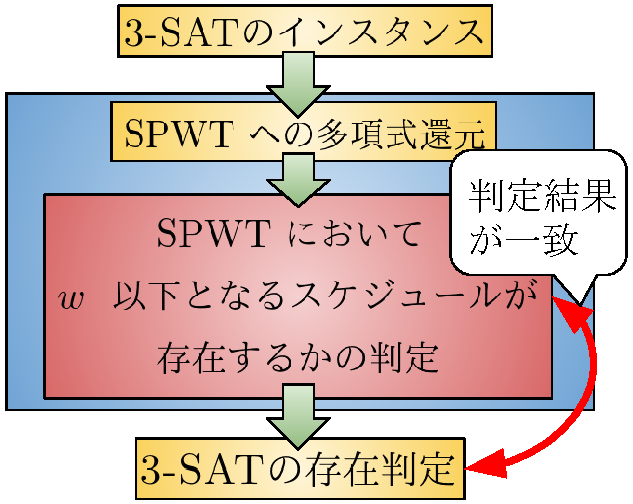
\includegraphics[width=7cm,bb=0 0 350 260]{figure/reduction.pdf}
          \end{textblock*}
        \end{minipage}
      \end{tabular}
      \begin{block}{}
        本研究では以下が成立することを示す.
        \begin{enumerate}
          \item スケジュールにおける最大待ち時間が $w$ 以下であるかの判定が\alert{多項式時間}で可能である.
          \item \textsc{3-SAT} のインスタンスから SWT のインスタンスが\alert{多項式時間}で構成可能であり,\textsc{3-SAT} の判定結果と構成したインスタンスに対する $w$ 以下となるスケジュールの存在判定結果が\alert{一致}する.
        \end{enumerate}
      \end{block}
    \end{frame}
    %%%%%%%%%%%%%%%%%%%%%%%%%%%%%%%%%%%%%%%%%%%%%%%%%%%%%%%%%%%%%%%%%%%
    % \section{多項式還元とは}
    % \begin{frame}{多項式還元とは:還元の流れ}
    %   \begin{block}{多項式還元}
    %     問題 $A$ の任意のインスタンスを,別の問題 $B$ のあるインスタンスに多項式時間で変換して,判定結果を同じにできるとき,
    %     \begin{center}
    %       「$A$ は $B$ に多項式還元可能」という.
    %     \end{center}
    %     \begin{itemize}
    %       \item $B$ を解くアルゴリズムを用いて,$A$ も解くことができるため,$B$ は $A$ と同等か,より難しいことがわかる.
    %     \end{itemize}
    %   \end{block}
    %   \begin{tabular}{cc}
    %     \begin{minipage}[]{0.5\hsize}
    %       本研究では,
    %       \begin{itemize}
    %         \item $A = {\mbox {\sc 3-SAT}}$
    %         \item $B = $ SWT の判定問題
    %       \end{itemize}
    %       として,SWT の NP 完全性を示した.
    %     \end{minipage}
    %     \begin{minipage}[]{0.5\hsize}
    %
    %     \end{minipage}
    %   \end{tabular}
    % \end{frame}
    % %%%%%%%%%%%%%%%%%%%%%%%%%%%%%%%%%%%%%%%%%%%%%%%%%%%%%%%%%%%%%%%%%%%
    \section{問題の分析}
    \begin{frame}{問題の分析:既存のスケジューリング問題との対応}
      \begin{block}{既存のスケジューリング問題との共通部分}
        \begin{itemize}
          \item {$w = 0$ のとき,処理開始可能時刻ちょうどで処理を開始しなければならない.}
          \begin{itemize}
            \item {\alert{JIT ジョブスケジューリング問題}と対応する.}
          \end{itemize}
          \item {SWT において,納期 = (処理開始可能時刻 + 処理時間 + $w$ )と定義できる.}
          \begin{itemize}
            \item {\alert{処理開始可能時刻と納期付きスケジューリング問題}と対応する.}
          \end{itemize}
        \end{itemize}
      \end{block}
      \begin{block}{既存のスケジューリング問題との差分}
        \begin{itemize}
          \item {SWT は,JIT ジョブスケジューリング問題の\alert{拡張問題}として捉えることができる.}
          \item {SWT は,処理開始可能時刻と納期付きスケジューリング問題の\alert{部分問題}として捉えることができる.}
        \end{itemize}
      \end{block}
      \begin{itemize}
        \item ${\mbox {JIT ジョブスケジューリング問題}} \subseteq {\mbox {SWT}}$
        \item ${\mbox {SWT}} \subseteq {\mbox {処理開始可能時刻と納期付きスケジューリング問題}}$
      \end{itemize}
    \end{frame}

    \begin{frame}{問題の分析:既存のスケジューリング問題の計算複雑さ}
      本研究では,JIT ジョブスケジューリング問題の 1 つである,
      \alert{JIT ジョブ荷重和最大化問題(SJIT)}と 処理開始可能時刻,納期付きスケジューリング問題の 1 つである\alert{処理開始可能時刻付き最大遅れ時間最小化問題(SRTD)}を SWT と対応付けた.
      \begin{block}{既存のスケジューリング問題の計算複雑さ}
        \begin{itemize}
          \item SJIT は,{\sc 3-SAT} からの還元により,無関連並列機械モデルにおいて,機械数が入力の一部の場合,\alert{強 NP 困難}である.
          \item SRTD は,{\sc 3-PARTITION} からの還元により,単一機械モデルにおいて,\alert{強 NP  困難}である.
        \end{itemize}
      \end{block}
    \end{frame}
    %%%%%%%%%%%%%%%%%%%%%%%%%%%%%%%%%%%%%%%%%%%%%%%%%%%%%%%%%%%%%%%%%%%
    \section{研究成果}
    \begin{frame}{研究成果:問題の計算複雑さ}
      \begin{alertblock}{成果 1}
        無関連並列機械モデルにおいて,機械数が入力の一部の場合,SWT が NP 完全であることを明らかにした.
      \end{alertblock}
      \begin{block}{インスタンスの変換}
        {\sc 3-SAT} のインスタンス を $X = \{x_1,\ldots,x_n\}$ と $H = \{h_1,\ldots,h_{\lambda}\}$ からなる 2 項組 $(X,H)$ とする.
        $(X,H)$ に基づき表記を導入する.
        \begin{itemize}
          \item $\forall i \in \{1,\ldots,n\},~\alpha_i = |\{h \in H \mid x_i \in h\}|$
          \begin{itemize}
            \item $H$ において,$x_i$ が現れる回数を表す自然数.
          \end{itemize}
          \item $\forall i \in \{1,\ldots,n\},~\beta_i = |\{h \in H \mid \bar x_i \in h\}|$
          \begin{itemize}
            \item $H$ において,$\bar x_i$ が現れる回数を表す自然数.
          \end{itemize}
          \item $\mathcal{A} = {\displaystyle \sum_{i \in \{1,\ldots,n\}}\alpha_i}$,$\mathcal{B} = {\displaystyle \sum_{i \in \{1,\ldots,n\}}\beta_i}$
        \end{itemize}
      \end{block}
      $2(\mathcal{A} + \mathcal{B}) + \lambda$ 個のジョブ $\mathcal{J}$ を $n + \lambda$ 台の無関連機械 $\mathcal{M}$ で処理する.
      ただし,$\mathcal{J} = \{\mathcal{J}^t,\mathcal{J}^f,\mathcal{J}^d\}$ s.t. $|\mathcal{J}^t| = |\mathcal{J}^f| = \mathcal{A} + \mathcal{B}$,$|\mathcal{J}^d| = \lambda$ とする.
    \end{frame}

    \begin{frame}{研究成果:問題の計算複雑さ}
      各 $i \in \{ 1,\ldots,n\}$ において,$\alpha_i \ge 3$,$\beta_i \ge 3$ のとき,次のように SWT のインスタンスを設定する.
      \begin{block}{各リテラルに対応するジョブの処理開始可能時刻の範囲}
        \begin{figure}[h]
          \centering
          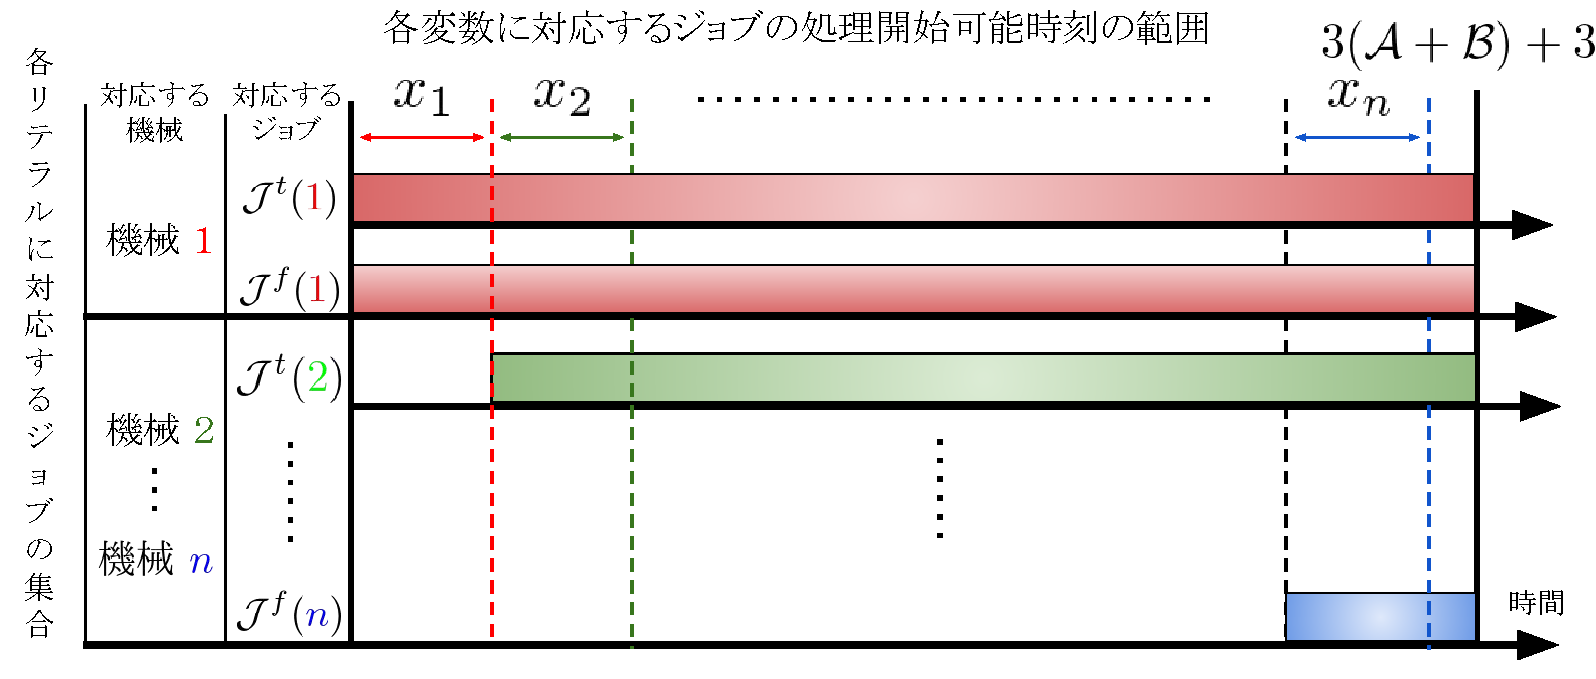
\includegraphics[width = 10 cm]{figure/3SAT3.pdf}
        \end{figure}
      \end{block}
      \begin{itemize}
        \item 各リテラルに対応するジョブの集合における各ジョブの処理開始可能時刻を,対応する機械ごとに範囲をずらして設定している.
        \item 各リテラルに対応するジョブの集合の中で,処理開始可能時刻が一番遅いジョブの完了時間は,$3(\mathcal{A} + \mathcal{B}) + 3$ と設定している.
      \end{itemize}
    \end{frame}

    \begin{frame}{研究成果:問題の計算複雑さ}
      \begin{block}{機械に対応するジョブを割り当てたときのスケジュール}
        \begin{figure}[h]
          \centering
          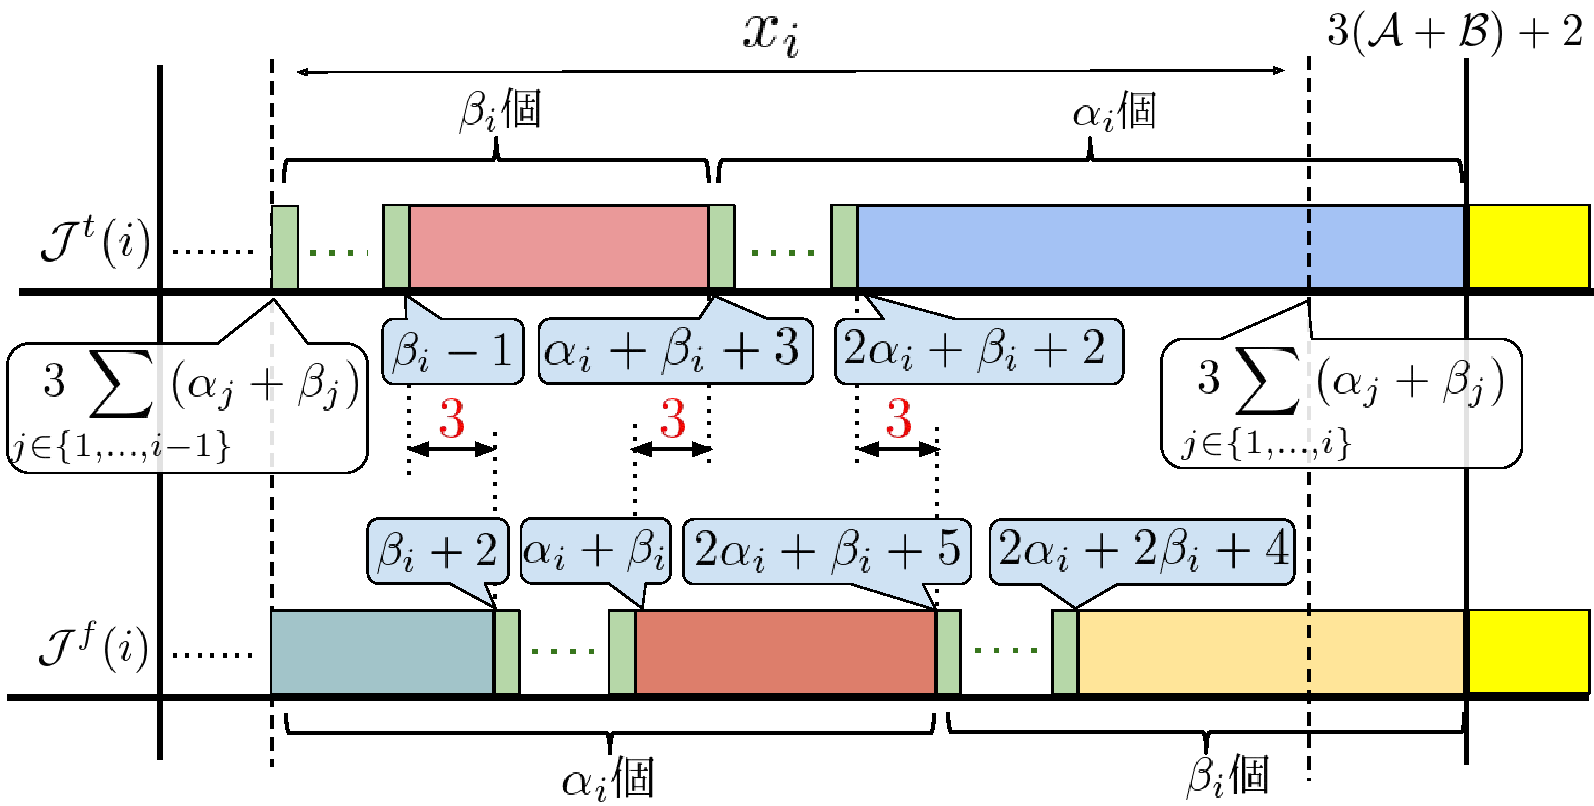
\includegraphics[width = 11cm]{figure/3SAT4.pdf}
        \end{figure}
      \end{block}
      \begin{itemize}
        \item $x_i$ と $\bar x_i$ に対応するジョブの集合 $\mathcal{J}^t(i)$ と $\mathcal{J}^f(i)$ におけるジョブ間の処理開始可能時刻の差を $3$ に設定している.
      \end{itemize}
    \end{frame}



    \begin{frame}{研究成果:問題の計算複雑さ}

      {\sc 3-SAT} の判定結果と,SWT における最大待ち時間が \alert{2 以下}となるスケジュールの存在判定結果が一致することを示した.

      \begin{block}{還元のポイント}
        \begin{itemize}
          \item {\sc 3-SAT} の判定結果が \alert{Yes} のとき,SWT における最大待ち時間は \alert{2 以下}になる .
          \item {\sc 3-SAT} の判定結果が \alert{No} のとき,SWT における最大待ち時間は \alert{3 以上}になる .
        \end{itemize}
      \end{block}
      無関連並列機械モデルにおいて機械数が入力の一部の場合,SWT が NP 困難である限り,$1.5$ 未満の定数近似アルゴリズムは存在しない.
    \end{frame}

    \begin{frame}{研究成果:ヒューリスティックの提案}
      \begin{alertblock}{成果 2}
        同一並列機械モデルにおける SWT に対して,ヒューリスティックの開発と解法に対する実験的評価を行った.
      \end{alertblock}
      \begin{block}{貪欲アルゴリズムに基づいた解法}
        \begin{description}
          \setlength{\leftskip}{-10mm}
          \item[入力 :] $I = (\mathcal{J}, \mathcal{M},r,p,C)$
          \item[出力 :] スケジュールの集合 $\mathcal{S}$.
          \begin{description}
            \setlength{\leftskip}{-25mm}
            \item[Step 1.]
            $\mathcal{J}$ を処理開始可能時刻の昇順でソートする.
            \item[Step 2.]
            各 $1 \le i \le n$ における $J_i$ について以下の処理を繰り返す.
            \begin{description}
              \item[Step 2.1.]
              \setlength{\leftskip}{-40mm}
              最小完了時刻を持つスケジュール集合の要素 $S_{M_a} \in \left\{ \displaystyle \argmin_{M \in \mathcal{M}}C(S_M)\right\}$ を 1 つ求める.
              ここで,$S_{M_a} := S_{M_a} \cup J_i$ とする.
            \end{description}
            \item[Step 3.]
            $\mathcal{S} = \{ S_M \mid M \in \mathcal{M}\}$ として,$\mathcal{S}$ を出力する.
          \end{description}
        \end{description}
      \end{block}
    \end{frame}

    \begin{frame}{研究成果:ヒューリスティックの精度について}
      ヒューリスティックから得られた解の最大待ち時間と厳密解法から得られた解の最大待ち時間の比に着目して比較を行った.
      \begin{exampleblock}{例:2 台の同一機械と以下のインスタンスにおけるスケジュール}
        \begin{tabular}{cc}
          \begin{minipage}[]{0.6\hsize}
            最適なスケジュール $S_1, S_2 \in \mathcal{S}$ は,
            \begin{itemize}
              \item $S_1:(J_1,J_3,J_5)$,$S_2:(J_2,J_4,J_6)$.
              \item $\mathcal{S}$ における最大待ち時間は $0$.
            \end{itemize}
            最適でないスケジュール $S'_1, S'_2 \in \mathcal{S'}$ は,
            \begin{itemize}
              \item $S'_1:(J_1,J_3,J_6)$,$S'_2:(J_2,J_4,J_5)$.
              \item $\mathcal{S'}$ における最大待ち時間は $3$.
            \end{itemize}
          \end{minipage}
          \begin{minipage}[c]{0.4\hsize}
            \begin{table}[htb]
              \begin{tabular}{|l|c|r|} \hline
                $\mathcal{J}$ & $r(J)$ & $p(J)$ \\ \hline \hline
                $J_1$ & 2 & 8 \\ \hline
                $J_2$ & 3 & 7 \\ \hline
                $J_3$ & 11 & 11 \\ \hline
                $J_4$ & 16 & 10 \\ \hline
                $J_5$ & 23 & 10 \\ \hline
                $J_6$ & 26 & 11 \\ \hline
              \end{tabular}
            \end{table}
          \end{minipage}
        \end{tabular}
        ${\displaystyle \frac{\text{ヒューリスティックから得られた解の最大待ち時間}}{\text{厳密解法から得られた解の最大待ち時間}} = \infty}$
      \end{exampleblock}
      本研究で提案したヒューリスティックは,上記の比が定数となることが保証されている.
    \end{frame}

    \begin{frame}{研究成果:ヒューリスティックの実験的評価}
      \begin{itemize}
        \item 実験回数:約 $300$ 万回
        \item 縦軸:$\frac{\text{ヒューリスティックから得られた解の最大待ち時間}}{\text{厳密解法から得られた解の最大待ち時間}}$
        \item 横軸:
      \end{itemize}
      % \begin{figure}[h]
      %   \centering
      %   \includegraphics[width = 12cm]{figure/}
      % \end{figure}
    \end{frame}

    \begin{frame}{研究成果:厳密解法の提案}
      \begin{alertblock}{成果 3}
        同一並列機械モデルにおける SWT に対して,厳密解法の開発と計算時間の分析を行った.
      \end{alertblock}
      % 厳密解法に\alert{分割生成アルゴリズム}と\alert{分枝限定法アルゴリズム}を用いた.
      % 以下の改良を加え,計算効率を向上させた.
      \begin{block}{分割生成アルゴリズムの改良}
        \begin{itemize}
          \item \alert{分割の要素数 = 機械数} となる分割のみ生成するように改良.
          \begin{itemize}
            \item 考慮する分割の数を減らすことができる.
          \end{itemize}
        \end{itemize}
      \end{block}
      \begin{block}{分枝限定法アルゴリズムの改良}
        \begin{itemize}
          \item \alert{部分問題に対する多項式アルゴリズム}の概念を導入した.
          \begin{itemize}
            \item 列挙する実行可能解を減らすことができる.
          \end{itemize}
        \end{itemize}
      \end{block}
      \begin{block}{上記以外の改良}
        \begin{itemize}
          \item 各機械におけるスケジュールのコストの降順で,探索を始める.
          \begin{itemize}
            \item 各分割における探索初期段階で,探索の中断を判定できる.
          \end{itemize}
        \end{itemize}
      \end{block}
    \end{frame}

    \begin{frame}{研究成果:分割生成アルゴリズムの改良}
      \begin{block}{}
        \uncover<1->{
        \alert{同一並列機械モデル}において,ジョブ $J_1$ を機械 $1$ に割り当てるのと,機械 $2$ に割り当てることは同じである.
        したがって,ジョブをどの機械に割り当てるかではなく,\alert{どのジョブと同じ機械に割り当てるか}を考える必要がある.
        つまり,同一並列機械モデルにおけるジョブの機械への割り当ては,\alert{ジョブの分割}として捉えることができる.
        }
      \end{block}
      \begin{exampleblock}{例:ジョブ数 3,同一機械数 2 における分割}
        \begin{figure}[h]
          \centering
          \includegraphics<1>[width = 12cm]{figure/rgf1.pdf}
          \includegraphics<2>[width = 12cm]{figure/rgf2.pdf}
          \includegraphics<3>[width = 12cm]{figure/rgf3.pdf}
          \includegraphics<4>[width = 12cm]{figure/rgf4.pdf}
        \end{figure}
      \end{exampleblock}

    \end{frame}
    \begin{frame}{分割生成アルゴリズムの改良による計算時間の評価}
      分割生成アルゴリズムの改良前と,改良後の計算時間の比較を行った.
      \begin{itemize}
        \item 実験回数:約 $3,000$ 回
        \item 縦軸:計算時間
        \item 横軸:
      \end{itemize}
      % \begin{figure}[h]
      %   \centering
      %   \includegraphics[]{}
      % \end{figure}
    \end{frame}

    \begin{frame}{分枝限定法アルゴリズムの改良}
      \begin{exampleblock}{例:以下のインスタンスにおけるスケジュール生成}
        \begin{tabular}{cc}
          \begin{minipage}[]{0.6\hsize}
            \begin{figure}[h]
              \centering
              \includegraphics<1>[width = 8cm]{figure/BandB1.pdf}
              \includegraphics<2>[width = 8cm]{figure/BandB2.pdf}
            \end{figure}
          \end{minipage}
          \begin{minipage}[c]{0.4\hsize}
            \begin{table}[htb]
              \begin{tabular}{|l|c|r|} \hline
                $\mathcal{J}$ & $r(J)$ & $p(J)$ \\ \hline \hline
                $J_1$ & 2 & 4 \\ \hline
                $J_2$ & 5 & 7 \\ \hline
                $J_3$ & 10 & 15 \\ \hline
              \end{tabular}
            \end{table}
          \end{minipage}
        \end{tabular}
      \end{exampleblock}
      \begin{itemize}
        \uncover<1>{
        \item それまでに割り当てたジョブのスケジュールにおける最大待ち時間がそれまでの最良の解 $W$ より良い値か?
        }
        \uncover<2>{
        \item 割り当てていない残りのジョブを最適にスケジュールしたときの最大待ち時間がそれまでの最良の解 $W$ より良い値か?
        \begin{itemize}
          \item SWT は,処理時間が一定のとき,処理開始可能時刻の昇順で処理することで最適解が求まる.
        \end{itemize}
        }
      \end{itemize}
    \end{frame}

    \begin{frame}{分枝限定法アルゴリズムの改良による計算時間の評価}
      分枝限定法アルゴリズムの改良前と,改良後の計算時間の比較を行った.
      \begin{itemize}
        \item 実験回数:約 $3,000$ 回
        \item 縦軸:計算時間
        \item 横軸:
      \end{itemize}
      % \begin{figure}[h]
      %   \centering
      %   \includegraphics[]{}
      % \end{figure}

    \end{frame}
    %%%%%%%%%%%%%%%%%%%%%%%%%%%%%%%%%%%%%%%%%%%%%%%%%%%%%%%%%%%%%%%%%%%
    \section{まとめと今後の課題}
    \begin{frame}{まとめと今後の課題}
      \begin{block}{まとめ}
        \begin{itemize}
          \item 無関連並列機械モデルにおいて,機械数が入力の一部の場合,SWT の NP 完全性を明らかにした.
          \begin{itemize}
            \item 1.5 未満の定数近似ができないことを明らかにした.
          \end{itemize}
          \item SWT に対するヒューリスティックと厳密解法の開発した.
          \item 実験的評価を行い,対象とする環境におけるヒューリスティックの有効性,厳密解法の有用性を示した.
        \end{itemize}
      \end{block}
      \begin{alertblock}{今後の課題}
        \begin{itemize}
          \item 無関連並列機械モデル以外の機械モデルにおける SWT の計算複雑さを明らかにし,問題の難しさに影響を与える特徴を明らかにする.
          \item {\sc 3-SAT} からの還元手法を工夫して,{\sc 3-SAT} の存在判定が Yes のとき,No のときの SWT の最大待ち時間の比を調整する.
          \begin{itemize}
            \item 上記の比を大きくすることができれば,その比未満の定数近似アルゴリズムが存在しないことを保証できる.
          \end{itemize}
          \item 上記の結果に基づき,近似アルゴリズムを開発する.
        \end{itemize}
      \end{alertblock}
    \end{frame}
    %%%%%%%%%%%%%%%%%%%%%%%%%%%%%%%%%%%%%%%%%%%%%%%%%%%%%%%%%%%%%%%%%%%
    \begin{frame}

    \end{frame}
    %%%%%%%%%%%%%%%%%%%%%%%%%%%%%%%%%%%%%%%%%%%%%%%%%%%%%%%%%%%%%%%%%%%
    \begin{frame}{付録:多項式還元の例({\sc 3-SAT} の判定結果が Yes のとき)}
      \begin{exampleblock}{例:各変数に対応する機械におけるスケジュール}
        $X = \{x_1,x_2,x_3\}$,$H = \big\{
        \{x_1,x_2,\bar x_3\},
        \{x_1,x_2,x_3\},
        \{x_1,\bar x_2,\bar x_3\},$
        \\
        $\{\bar x_1,x_2,x_3\},
        \{\bar x_1,\bar x_2,x_3\},
        \{\bar x_1,\bar x_2,\bar x_3\}
        \big\}$ の 2 項組 $(X,H)$ が {\sc 3-SAT} のインスタンスとして与えられたとき,前のスライドで説明した方法により,SWT のインスタンス $I_{(X,H)}$ を作る.
        \begin{itemize}
          \item $(X,H)$ において,$H$ を充足する真理値割り当ての 1 つ $f(x_1) = 1$,$f(x_2) = 0$,$f(x_3) = 1$ が存在する.
        \end{itemize}
        各 $i \in \{0,1,2\}$ における機械 $i$ 上のスケジュールは以下の通り.
        \begin{figure}[h]
          \centering
          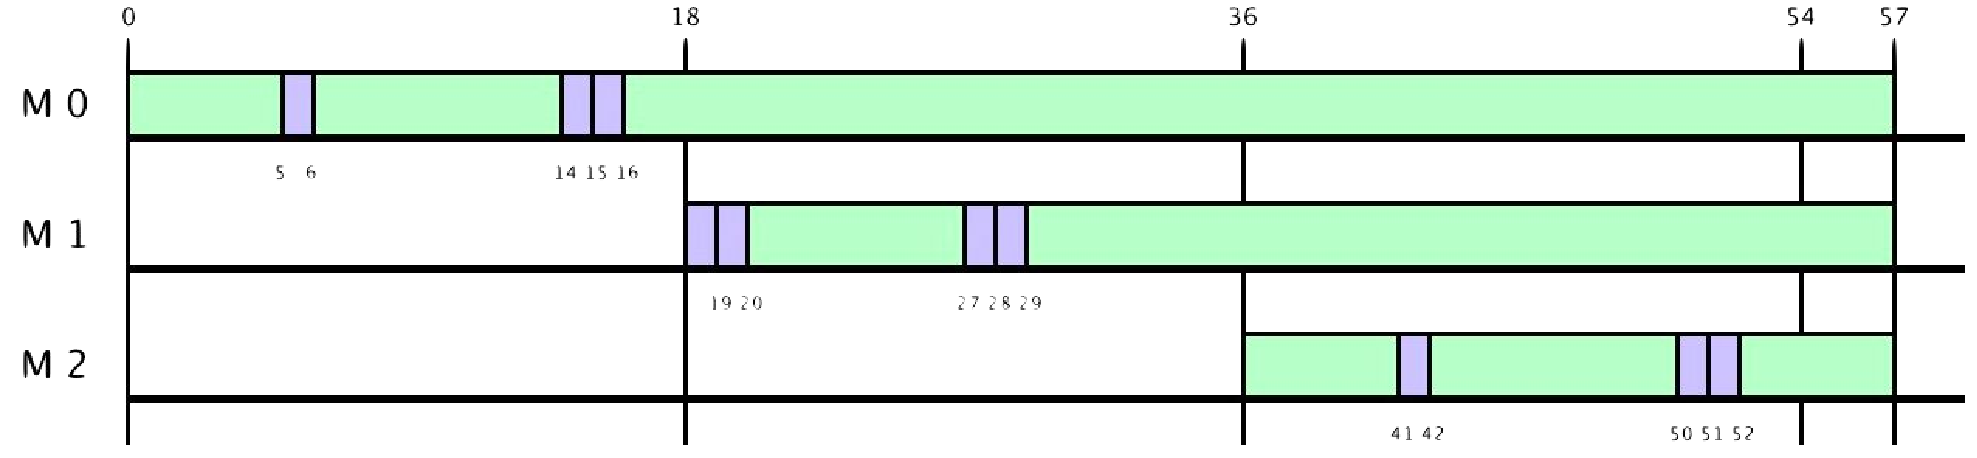
\includegraphics[width = 12cm]{figure/reductionExample1.pdf}
        \end{figure}
      \end{exampleblock}
    \end{frame}

    \begin{frame}{付録:多項式還元の例({\sc 3-SAT} の判定結果が Yes のとき)}
      \begin{exampleblock}{例:各節に対応する機械におけるスケジュール}
        $H$ を充足する真理値割り当てが存在することから,各節におけるリテラルのなかで,少なくとも 1 つ 1 (true) に割り当てられたジョブが存在する.

        したがって,各 $k \in \{3,\ldots,8\}$ における機械 $k$ に割り当てられた最後のジョブの待ち時間は高々 $2$ である.以下の通り.
        \begin{figure}[h]
          \centering
          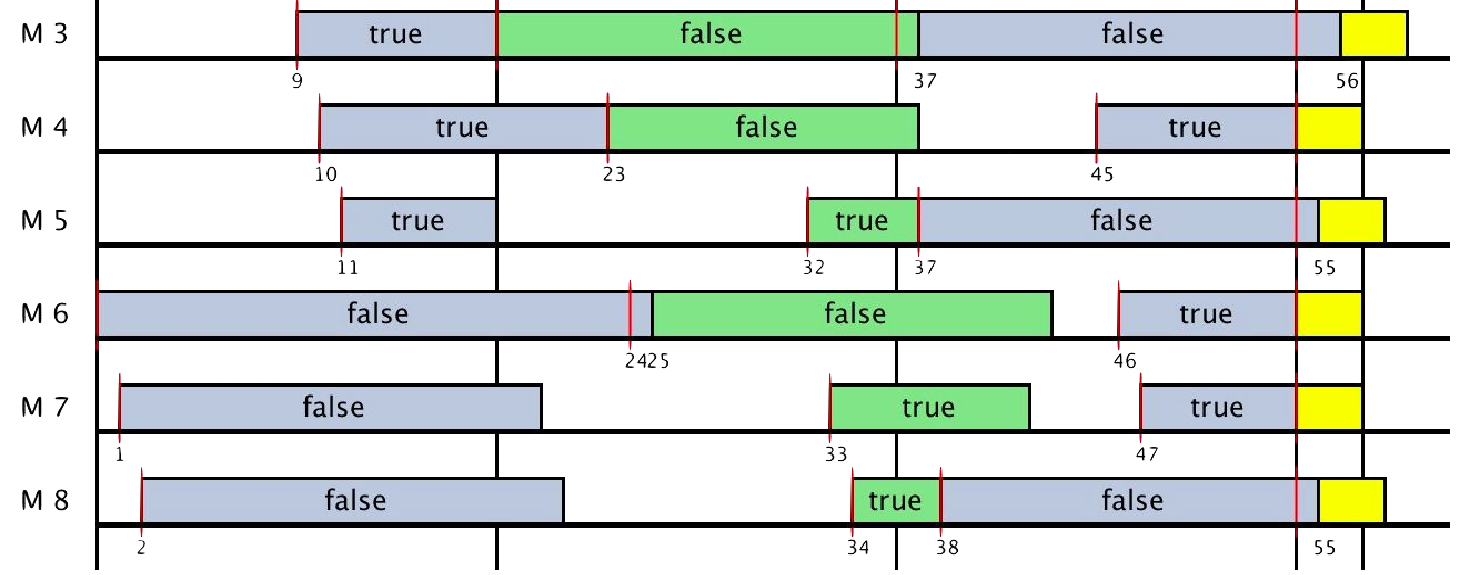
\includegraphics[width = 12cm]{figure/reductionExample2.pdf}
        \end{figure}
      \end{exampleblock}
    \end{frame}

    \begin{frame}{付録:多項式還元の例({\sc 3-SAT} の判定結果が Yes のとき)}
      \begin{exampleblock}{例:すべての機械におけるスケジュール}
        \begin{figure}[h]
          \centering
          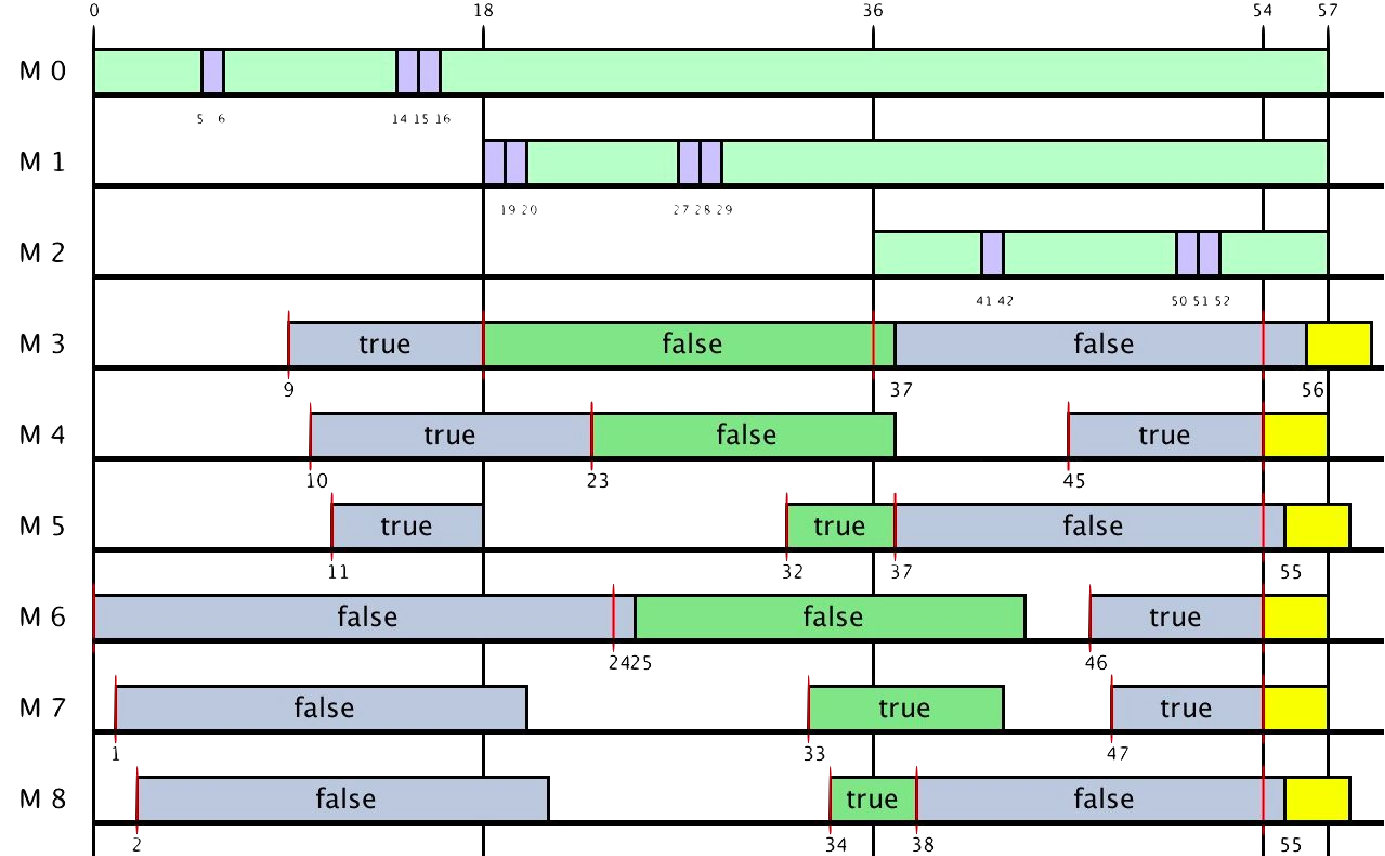
\includegraphics[width = 12cm]{figure/reductionExample3.pdf}
        \end{figure}
      \end{exampleblock}
    \end{frame}

    \begin{frame}{付録:多項式還元の例({\sc 3-SAT} の判定結果が No のとき)}
      \begin{exampleblock}{例:各変数に対応する機械におけるスケジュール}
        $X = \{x_1,x_2,x_3\}$,$H = \big\{
        \{x_1,x_2,x_3\},
        \{\bar x_1,\bar x_2,\bar x_3\},
        \{x_1,\bar x_2,\bar x_3\},$
        \\
        $\{\bar x_1,x_2,\bar x_3\},
        \{\bar x_1,\bar x_2,x_3\},
        \{\bar x_1,x_2,x_3\},
        \{x_1,\bar x_2,x_3\},
        \{x_1,x_2,\bar x_3\}
        \big\}$ の 2 項組 $(X,H)$ が {\sc 3-SAT} のインスタンスとして与えられたとき,前のスライドで説明した方法により,SWT のインスタンス $I_{(X,H)}$ を作る.
        \begin{itemize}
          \item $(X,H)$ において,$H$ を充足する真理値割り当ては存在しない.
          \item ここで,$f(x_1) = 1$,$f(x_2) = 1$,$f(x_3) = 1$ としたとき,
        \end{itemize}
        各 $i \in \{0,1,2\}$ における機械 $i$ 上のスケジュールは以下の通り.
        \begin{figure}[h]
          \centering
          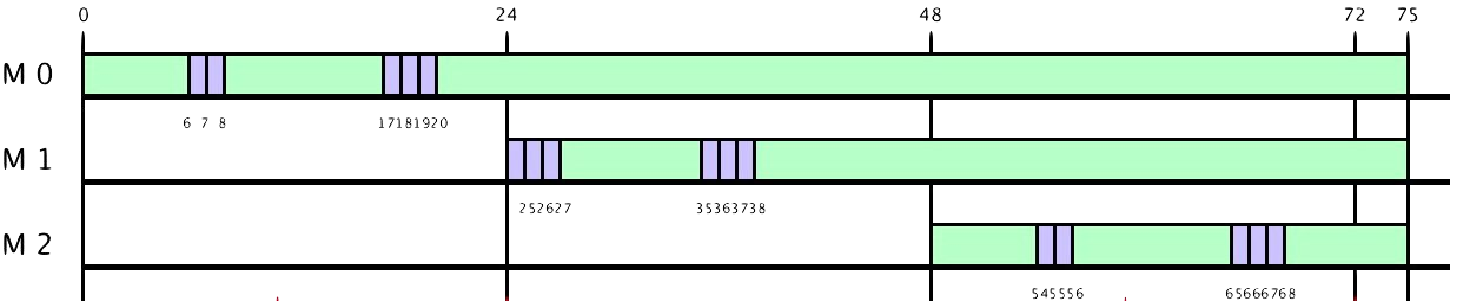
\includegraphics[width = 12cm]{figure/reductionExample4.pdf}
        \end{figure}
      \end{exampleblock}
    \end{frame}

    \begin{frame}{付録:多項式還元の例({\sc 3-SAT} の判定結果が No のとき)}
      \begin{exampleblock}{例:各節に対応する機械におけるスケジュール}
        $H$ を充足する真理値割り当てが存在しないことから,各節におけるリテラルのなかで,すベて 0 (false) に割り当てられたジョブが割り当てられた機械が少なくとも 1 つ存在する.

        したがって,各 $k \in \{3,\ldots,10\}$ における機械 $k$ に割り当てられた最後のジョブの待ち時間が $3$ 以上となる機械が存在する.以下の通り.
        \vspace{-4mm}
        \begin{figure}[h]
          \centering
          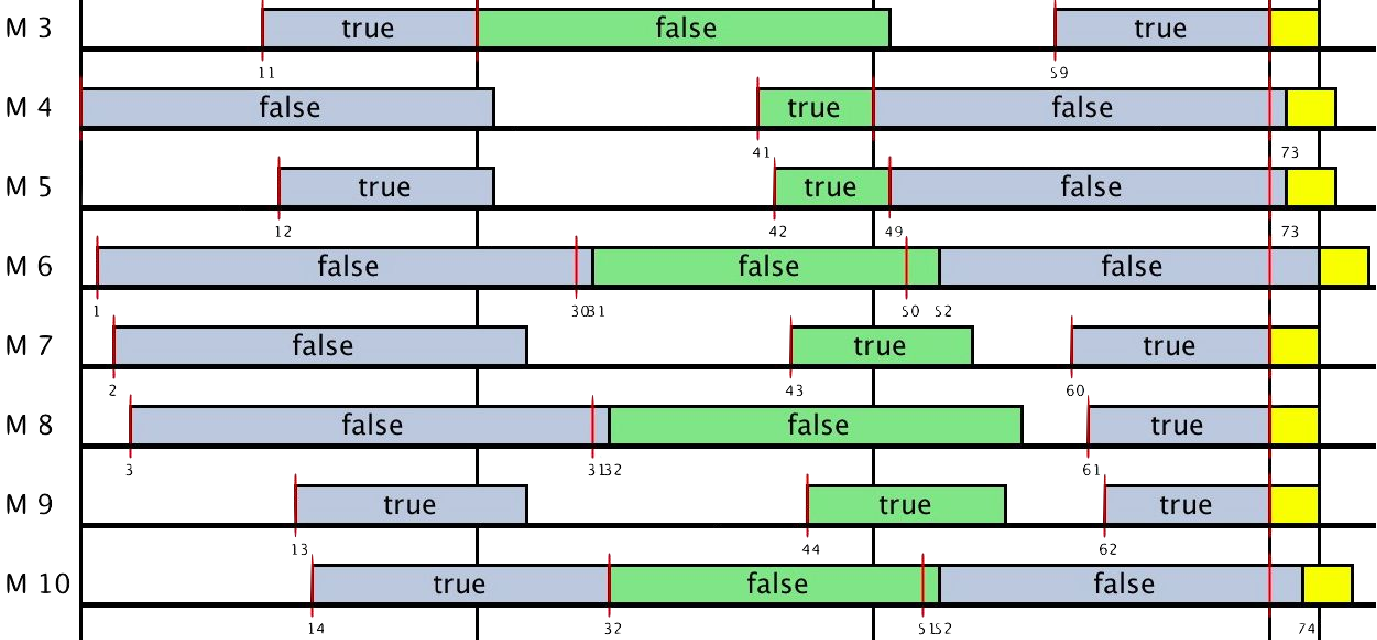
\includegraphics[width = 11cm]{figure/reductionExample5.pdf}
        \end{figure}
      \end{exampleblock}
    \end{frame}

    \begin{frame}{付録:多項式還元の例({\sc 3-SAT} の判定結果が No のとき)}
      \begin{exampleblock}{例:すべての機械におけるスケジュール}
        \begin{figure}[h]
          \centering
          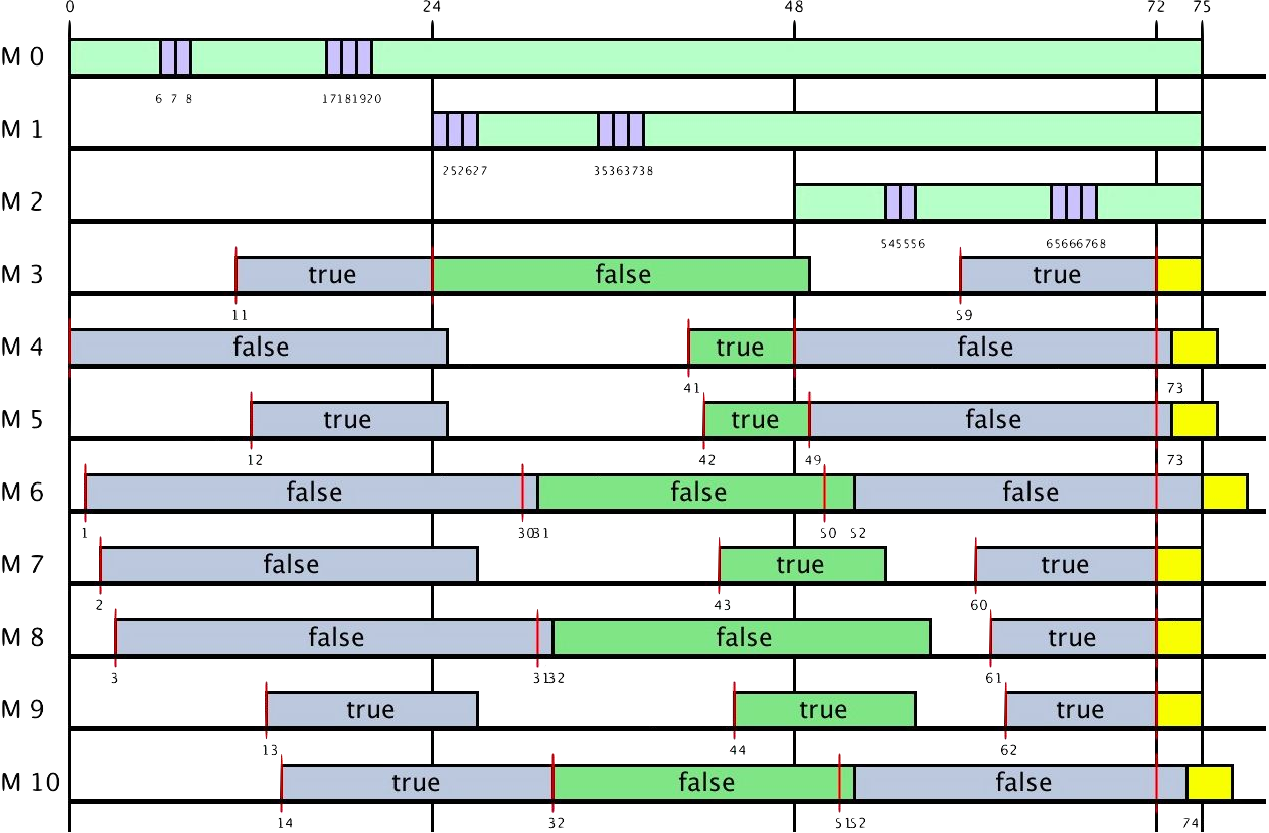
\includegraphics[width = 11cm]{figure/reductionExample6.pdf}
        \end{figure}
      \end{exampleblock}
    \end{frame}

    \begin{frame}{付録:多項式還元の例(特殊なケース)}
      \begin{block}{特殊なケースにおけるインスタンスの作り方}
        例えば,$X = \{x_1,x_2,x_3\}$,$H = \big\{{\color{red}\{x_1,x_2,\bar x_3\}},{\color{blue}\{\bar x_1, \bar x_2, \bar x_3\}}\big\}$ のとき,
        \begin{itemize}
          \item
          各 $i \in \{1,2,3\}$ に対して,$\alpha_i$,$\beta_i$ は 3 以下である.
          \item
          このとき,各 $i \in \{1,2,3\}$ に対して,$\alpha_i$,$\beta_i$ は 3 以上となるように,ダミーの節を作る.以下の通り.
        \end{itemize}
        \begin{equation}
          \begin{split}
            H &= \big\{
            {\color{red}\{x_1,x_2,\bar x_3\}},
            {\color{red}\{x_1,x_2,\bar x_3\}},
            {\color{red}\{x_1,x_2,\bar x_3\}},
            \\ & \qquad\qquad\qquad\qquad\qquad
            {\color{blue}\{\bar x_1, \bar x_2, \bar x_3\}},
            {\color{blue}\{\bar x_1, \bar x_2, \bar x_3\}},
            {\color{blue}\{\bar x_1, \bar x_2, \bar x_3\}}
            \big\} \notag
          \end{split}
        \end{equation}
        \begin{itemize}
          \item 作成したダミー節は,本来 $H$ の要素である節と同じ節を複数個用意したに過ぎない.そのため,真理値割り当てに関係なく,判定結果にも影響しない.
        \end{itemize}
        上記のように,ダミー節を含んだ節の集合を作り,その後の SWT のインスタンスへの変換する.インスタンスの変換方法は,前のスライドで記述した通り.
      \end{block}
    \end{frame}

    \begin{frame}{付録:ヒューリスティックの精度の保証の証明}

    \end{frame}

    \begin{frame}{付録:分割生成アルゴリズムの改良部分}

    \end{frame}

    \begin{frame}{付録:分枝限定法アルゴリズムの改良部分}
      \begin{block}{分枝限定法アルゴリズムの改良部分}
        \begin{description}
          \setlength{\leftskip}{-10mm}
          \item[入力 :] $I = (\mathcal{J'}, S)$
          \item[出力 :] スケジュール $S$.
          \begin{description}
            \setlength{\leftskip}{-25mm}
            \item[Step 1.]
            各 $1 \le i \le |\mathcal{J'}|$ における $J'_i$ について,以下の処理を繰り返す.
            \begin{description}
              \setlength{\leftskip}{-40mm}
              \item[Step 1.1.]
              $p(J'_i) = {\displaystyle \min_{j \in \{1,\ldots,|\mathcal{J'}|\}}p(J'_j)}$ とする.
              \item[Step 1.2.]
              $S := S \cup J'_i$ とする.
            \end{description}
            \item[Step 2.]
            $S$ を出力する.
          \end{description}
        \end{description}
      \end{block}
      \begin{itemize}
        \item Step 1. で $\mathcal{J'}$ におけるすべてのジョブの処理時間を $\mathcal{J'}$ の中の最小の処理時間に設定している.
        \item 上記の操作により,$\mathcal{J'}$ におけるジョブの本来の処理時間は,設定した処理時間以上である.
        \item このとき,処理開始可能時刻順で処理して得られるスケジュールにおける最大待ち時間は,$\mathcal{J'}$ におけるコストの下限である.
      \end{itemize}
    \end{frame}
    %%%%%%%%%%%%%%%%%%%%%%%%%%%%%%%%%%%%%%%%%%%%%%%%%%%%%%%%%%%%%%%%%%%
    \end{document}
